% !TEX root = ../main.tex
% !TEX spellcheck = en_US
\chapter{Results}
These are the results from testing the bot on 14 people, 12 males and 2 females, ages 21–26, with
skills varying from beginners who only played StarCraft a few times to those who have played more
than 20 hours of skirmish matches in either StarCraft: Brood War or StarCraft 2.

\begin{figure}[htb]
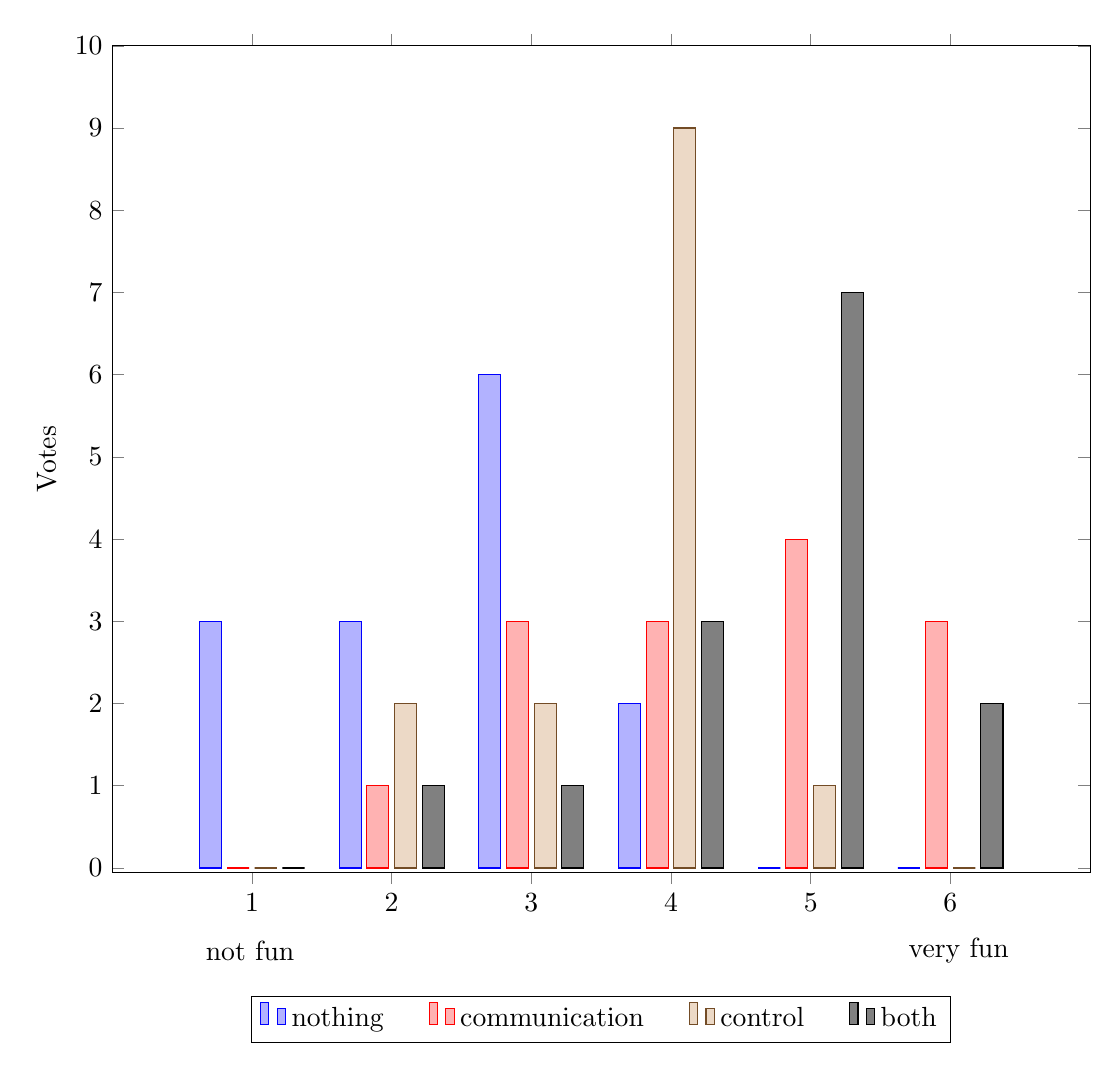
\begin{tikzpicture}
\begin{axis}[width=14cm,
	ylabel=Votes,
	ymin=-0.05,ymax=10,
	xmin=0,xmax=7,
	enlargelimits=false,
	xtick=data,
	legend style={at={(0.5, -0.15)},
		anchor=north, legend columns=-1,/tikz/every even column/.append style={column sep=0.5cm}},
	ybar,
	bar width=8pt,
]

% no control, no communication
\addplot
	coordinates {(1,3) (2,3) (3,6) (4,2) (5,0) (6,0)};

% no control, with communication
\addplot
	coordinates {(1,0) (2,1) (3,3) (4,3) (5,4) (6,3)};

% with control, no communication
\addplot
	coordinates {(1,0) (2,2) (3,2) (4,9) (5,1) (6,0)};

% with control, with communication
\addplot
	coordinates {(1,0) (2,1) (3,1) (4,3) (5,7) (6,2)};

\legend{nothing, communication, control, both};
\end{axis}
\node at (1.75,-1) {not fun};
\node at (10.75,-1) {very fun};
\end{tikzpicture}
\caption{Fun degree of the four scenarios}
\label{fig:results_fun}
\end{figure}

\def\scenarionames{{"None","Comm","Control","Comm+Cont"}}
\begin{figure}[htb]
	\centering
	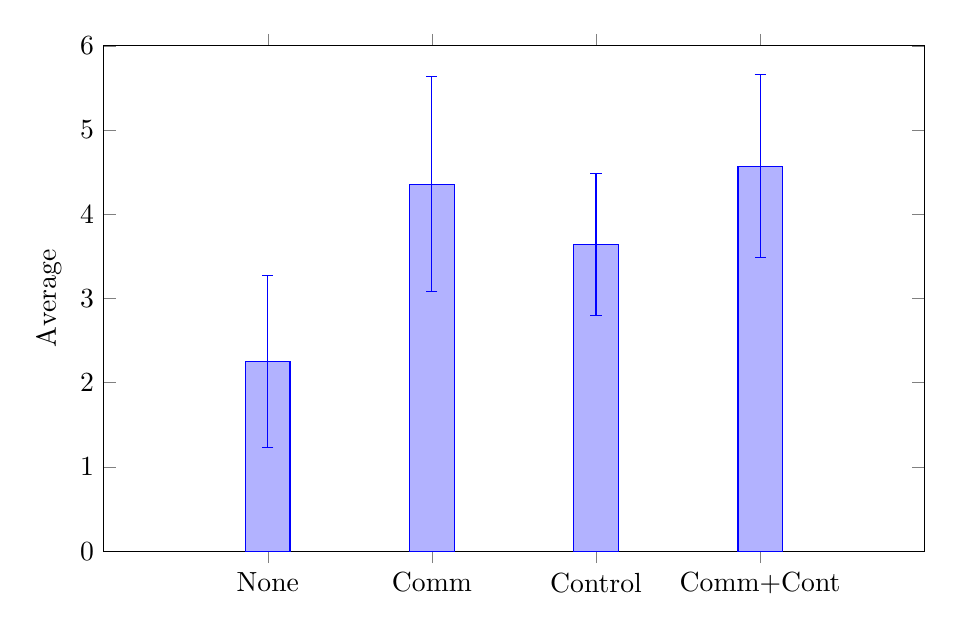
\begin{tikzpicture}
		\begin{axis}[width=12cm,height=8cm,
			ylabel=Average,
			xmin=-1,xmax=4,
			ymin=0,ymax=6,
			enlargelimits=false,
			legend style={at={0.5, -0.15)},
				anchor=north, legend columns=-1,/tikz/every even column/.append style={column sep=0.5cm}},
			ybar,
			bar width=16pt,
			xtick=data,
			xticklabel={\pgfmathparse{\scenarionames[Mod(\tick,4)]}\pgfmathresult},
		]
			
			\addplot+[error bars/.cd,y dir=both,y explicit]
				coordinates {
					(0, 2.25) +- (0, 1.019)
					(1, 4.357) +- (0, 1.277)
					(2, 3.643) +- (0, 0.842)
					(3, 4.571) +- (0, 1.089)
				};

		\end{axis}

	\end{tikzpicture}
	\caption{Average vote with standard deviation}
	\label{fig:results_average}
\end{figure}

\subsection{RQ 1 Which type of bot is most fun to play with?}
``Which is most fun to play with, communicating bot, controllable bot, both communicating and
controllable bot, or none?'' Figure \ref{fig:results_fun} shows the questionnaire results from the
four questions, one for each scenario; the results are summorized in figure
\ref{fig:results_average} for an easier comparison.

To validate our hypothesis if the testers thought it was most fun to play (in this order) with a communicating and
controllable, communicating, controllable, and a bot with none of these features we conducted paired two-sample
T-tests, results found in table \ref{tbl:t-test-all}. These null hypotheses tests whether the
differences between the scenarios are enough to deduct
whether the order from figure \ref{fig:results_average} could be trusted.

\begin{table}[htbp]
\begin{center}
\begin{tabular}{|c|c|c|c|c|}
\hline
 & \textbf{None} & \textbf{Comm} & \textbf{Control} & \textbf{Comm+Cont} \\ \hline
\textbf{None} & N/A & 0.0013 & 0.0029 & 0.0015 \\ \hline
\textbf{Comm} & 0.0013 & N/A & 0.1461 & 0.6301 \\ \hline
\textbf{Control} & 0.0029 & 0.1461 & N/A & 0.0094 \\ \hline
\textbf{Comm+Cont} & 0.0015 & 0.6301 & 0.0094 & N/A \\ \hline
\end{tabular}
\end{center}
\vspace{-12pt}
\caption{Paired two-sample t-test}
\label{tbl:t-test-all}
\end{table}
From table \ref{tbl:t-test-all} we can see that there is not enough difference between neither
communication + control and only communication nor only communication and only control. What we can
deduct from this the possible order of fun in table \ref{tbl:order_fun} where 1 is most fun and 4 is
least fun.

\begin{table}[htb]
	\centering
	\begin{tabular}{|l|l|l|l|}
		\hline
		\textbf{1} & Communication + Control & Communication & \\ \hline
		\textbf{2} & Communication + Control & Communication & Control \\ \hline
		\textbf{3} & Communication & Control & \\ \hline
		\textbf{4} & None & & \\ \hline

	\end{tabular}
	\caption{Possible fun order from the t-tests}
	\label{tbl:order_fun}
\end{table}

An interesting observation was that some testers preferred communication over both control and
communication. During the interviews we found a correlation between control and player skill—players
with higher skill tended to prefer control whereas lower skill players became overwhelmed by all
tasks, including the control of the bot.





\paragraph{Control \& communication}
during the interviews 8 of 14 testers felt it was most fun to play with the bot when it had both
communication and control on. Two of the tester could not decide whether only communication or both
communication and control was more fun, but one mentioned that s/he would liked control and
communication more than only communication if s/he had been better at the game. Below you can find
the testers' reasons why control and communication was most fun to play.
\begin{itemize}
	\item I could build up my army, order him to attack and join his attack.
	\item Easier to plan because he told me his plans.
	\item I could order him to attack where I attacked using the follow command.
	\item You get a direct response from him after an order—you know that something will happen.
	\item Nice to be able to control him.
	\item It was fun that he explained his strategies.
\end{itemize}

\paragraph{Communication only}
6 of 14 testers (including the two testers already mentioned that could not decide on whether only
communication or both communication and control was most fun) thought it was most fun to play with
the bot when it only had communication on. Below you can find the testers' reasons why communication
was most fun to play.
\begin{itemize}
	\item I already had a lot on my mind, controlling him was a bit too much for me.	
	\item Easier for me to plan because he told me his plans.
	\item I am lazy therefore it was easier to let the bot do the hard work.
\end{itemize}

\paragraph{Control only}
2 of 14 testers thought it was most fun to play only with control. Although these might not be
credible as for one tester it was the only game s/he won in the test and s/he told us that it was
only because of that it was most fun, otherwise s/he guessed it would be more fun with
communication. The other tester only thought control was most fun as it was the first scenario s/he
tested, otherwise s/he thought control and communication was most fun because ``it was easier to play
when I (the tester) can send attacks at the same time his and it gets easier to see what the bot
does'' (paraphrased), i.e. same reasons as other players who thought control and communication was most fun.

\subsection{RQ 1.1 Which features are most liked?}
Below the most liked features are shown in two lists, one containing general features and the other
specific commands they liked. As mentioned these can serve as guidelines for future work what
features shall be prioritized.
\paragraph{General liked features}
Most noteworthy is the communication which more than half of the testers commented on, more
specifically ``Fun to know what the bot is doing'' and ``Easier to plan because he told me his
plans.''
\begin{itemize}
	\item Communication
	\begin{itemize}
		\item He said why attacked, expanded, and so forth—I could learn from his strategies.
		\item Fun to know what the bot is doing.
		\item Easier to plan because he told me his plans.
		\item Feels more like team play when he is communicating.
		\item Direct response after ordering a command, then you knew if the bot would follow the command or not.
		\item It had humor, e.g. Leeeeroooooooy Jenkins message when attacking.
		\item Almost like playing with a real player.
		\item Asked player for help when under attack.
	\end{itemize}
	\item Uses same strategies as humans, such as attacking when expanding.
	\item Very good macro, always has much more units than me.
	\item Own initiative to do things.
	\begin{itemize}
		\item Followed me when I wanted to attack, even though I did not order him—feeling that I play with someone.
		\item Very good at expanding, and often.
		\item I could plan after how it acted and collaborate.
	\end{itemize}
	\item Coordinated defense—came and defended me when I needed help.
	\item It did not run its own race, I felt more involved in its decisions.
	\item Built tanks—I could back with my units and the tanks would clear the enemy units.
	\item Its attack cleared the path for me.
\end{itemize}

\paragraph{Liked commands}
\begin{itemize}
	\item Follow
	\begin{itemize}
		\item Doubles the amount of army size at one place.
		\item I did not have to attack by myself.
		\item Easier to coordinate where he should attack.
	\end{itemize}
	\item Attack
	\begin{itemize}
		\item I do not have to attack at the same place with my army.
		\item He could clear the path for me.
		\item Easy to reinforce as one could spam the attack button.
		\item He always had an army, if he attacked I could support him with my smaller army.
		\item He decided where to attack and I could follow and attack somewhere close.
	\end{itemize}
	\item Expand
	\begin{itemize}
		\item I like to control the timing between when I attack and he shall expand.
		\item I could order him to expand twice if the opportunity came, or just to expand when he did not notice he could expand.
	\end{itemize}
	\item Scout
	\begin{itemize}
		\item I do not have to scout and that is good as I am lazy.
	\end{itemize}
\end{itemize}

\subsection{RQ 1.2 Which features are most disliked?}
Instead of asking what features the testers disliked, we asked what they disliked about BATS (notice
the removal of feature). Below is a list of all things they disliked about BATS.
\paragraph{General disliked features}
Almost all testers mentioned they were annoyed by BATS halting its army in choke points making it
impossible for them to pass.
\begin{itemize}
	\item The army halted in choke points and made it impossible for me to come through.
	\item Got stuck when moving to a place, he ran back and forth until he finally ran more too long
		to the other side—note: regroup behavior.
	\item It did not follow me very well—note: when the squad it followed became very small (1-2
		units) the player did not notice it had units that the bot followed with 30+ units.
	\item Bot asks for help when few units attack and he can easily handle it.
	\item Felt like it changed how good it was during each scenarios.
	\item He attacked cowardly, slow attack with siege tanks instead of just marching in and killing
		everything which he could do in most situations.
	\item Sends too many messages at the same time, maybe queue up messages instead?—note: sometimes
		the bot will decide to retreat, but decides to attack directly after and then expand
		because it is attacking, thus 3 messages are printed directly after each other which can
		confuse the player..
	\item Never had units for drops.
	\item When it dropped it did not function very well.
	\item A better scout that scouted bases and not random locations.
\end{itemize}

\paragraph{Disliked commands}Two answered drop as it did not work properly, but most of the testers did not test all commands and thus could not answer if they disliked any command.

\subsection{RQ 1.3 Which features are missing?}
The testers were asked which features they missed during their scenarios, the first list presented
includes general features whereas the second list are specific commands they missed. These can serve
as guidelines for future developers what players want from a teammate bot.
\paragraph{General missed features}
\begin{itemize}
	\item More strategies, e.g. rush attacks, and would know about timings to make use of them.
	\item Use a variety of strategies depending on my build order.
	\item Give resources to the bot.
	\item Did not specify where he is under attack, would help me find the place.
	\item BATS could communicate what it thinks the player should do when s/he does not know what to do.
	\item More variety of units, more detection units.
	\item Scans in enemy bases.
	\item For the bot to play other races than Terran.
\end{itemize}

\paragraph{Missed commands, or improved existing commands}
\begin{itemize}
	\item A help button when the bot shall come and help me.
	\item Using way points for attacks to specify from where he should attack, either to not block my path or to create a more advanced attack.
	\item Drunken mode, random behavior.
	\item Command buttons grayed out when player could not use them.
	\item Retreat command.
	\item Abort command to abort the last command if the player misclicked.
	\item Hold position.
\end{itemize}

\subsection{Other questions and comments}
\paragraph{What surprised you in a positive way?}
A common misconception was that the testers would play against the bot and not with it. They thought
BATS was a good bot, that built up his army fast and that the tester did not need to babysit it.
They tended to like the funny messages, especially Leeeeeerrooooooy Jenkins. Common for many testers
were that the bot expanded just before they were going to send the expand command, which made them
think the bot was good at expanding and had a good timing on expands. A tester liked the underlying
reason behind each intention and not just the intention as s/he could learn from this. Another
tester was surprised by that it worked so well to play with a bot as they can be quite stupid.

\paragraph{What surprised you in a negative way?}
More than half of the testers thought BATS crowded the places he attacked and made it impossible to
bypass unless you had air units, 2 testers even changed their strategy to only air units because of
this. He did not clear the entire base as humans would do, but left the base when few buildings were
left. Twice the bot expanded to a location the player already expanded to, i.e. build a command
center beside their command center (or equal building). Sometimes the bot followed a small army
consisting of 1-2 units, this surprised the player as s/he thought it would either retreat or continue
attacking on its own.

\paragraph{If you won or lost, did you think it was because of you, BATS, or both?}
This question was not asked until the 6th tester, thus only 8 of 14 testers were asked this
question. Four of the tester thought they won because of both, where one of these thought it was
because of him/her in one of the four scenarios. Their reasons were that BATS was better at building
units, but they themselves had a better idea of strategy, where and how to attack. Two of the
testers thought it always because of them as they felt better than BATS, these two were amongst the
better players and also preferred control—a side note, there were two other players just as good as
them, one of them thought it was because of both and strangely the other thought it was because of
the bot. Another tester thought they won because of the bot as it had saved him/her at a very
crucial moment.

Only one loss occurred for the last 8 tester. The tester who lost felt that it was entirely
his/her fault as the bot had been attacked for 4 minutes and was defeated before the tester even
noticed it, although s/he mentioned that if the bot had said it was under attack it would never have
happened.

\paragraph{Commands used}
We noticed that many of the testers did not use all commands, no-one used the transition command as
all felt the bot handled that fairly well. Only a few (2–4) used the drop, expand, and scout
commands, with the same reason here as they felt the bot did a good job on this, except drop but
they did not feel as a drop was needed.

\paragraph{Other noteworthy comments}
One tester mentioned the bot felt like Brother in Arms where you can control other units. Another
tester mentioned that it was more fun to play with this bot than any other s/he had played with. A
third tester thought BATS could be used either when one wanted to play a regular co-op game but did
not have any friend to play with, or to fill an uneven team when playing with friends.

\subsection{Questions and comments about the experiment}
These are questions asked about the experiment itself and not directly associated with the bot.

\paragraph{Was the experiment fun or boring, and why?}
All testers thought it was fun to test the bot, both because StarCraft is a fun game and because it
was a new experience for many to play with a bot that you could control and communicate.

\paragraph{Was the experiment too long?}
The experiment was estimated to take 2 hours. Some testers thought it sounded quite long, but none
of the testers thought it was too long. Their reasons were that the scenarios were short (max 20
minutes) and they had fun testing the bot making time pass very quickly.

\paragraph{Other comments}
A tester commented how much difference there were between bots with and without communication, put
in the testers own words: ``I noticed how important the communication was and how bad something can
be when a feature is missing.''\footnote{Translated from Swedish ``Jag märkte hur viktig
kommunikationen var och hur dåligt någonting kan vara utan en feature''}
